\appendix
\renewcommand{\theequation}{A.\arabic{section}.\arabic{equation}}
\setcounter{equation}{0}

\section{物理数学}

\subsection{norm}

$\mathbb{R}^n$または
$\mathbb{C}^n$上の
$n$次元vector $v$に対し、
実数$1\le p < \infty$の範囲で
$L^p$-normを
\begin{align}
    ||v||_p
:=
    \left(
        \sum_{i=1}^n
        |v_i|^p
    \right)^{ \dfrac{1}{p} }
\end{align}
と定義する。
$p\to\infty$の極限を
$L^\infty$-normないし最大値normと言い、
\begin{align}
    ||v||_\infty
=
    \max_i
    |v_i|
\end{align}
に一致する。
特に$n \to \infty$(つまり無限数列)の場合、
上の$p$-normを有限にするようなvectorの集合を$l^p$と呼ぶ。

測度空間についても
和を積分に置き換えることにより同様のnormが定義でき、
これを有限にする可測関数の集合を
$L^p$空間と呼ぶ。

\subsection{$\Gamma$関数}

$\Gamma$関数は$\Re z > 0$の複素数$z$に対し
\begin{align}
    \Gamma(z)
    := \int_0^\infty dt t^{z-1} e^{-t}
\end{align}
により定義され、
その性質
$\Gamma(1) = 1, \Gamma(z+1) = z\Gamma(z)$
から階乗
\begin{align}
    \Gamma(n+1) &= n!
\end{align}
の複素数への一般化を与える。

\subsection{複素関数}

\subsubsection{Laurent series expansion(ローラン級数展開)}

\begin{wrapfigure}[7]{r}[5pt]{107pt}
  \centering
  

\tikzset{every picture/.style={line width=0.75pt}} %set default line width to 0.75pt        

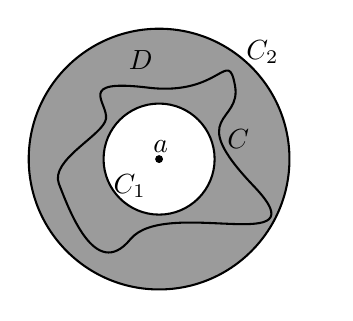
\begin{tikzpicture}[x=0.4pt,y=0.4pt,yscale=-1,xscale=1]
%uncomment if require:
\path (0,240.79999542236328);
%set diagram left start at 0, and has height of 240.79999542236328

%Shape: Circle [id:dp6258198346024846] 
\draw  [fill={rgb, 255:red, 155; green, 155; blue, 155 }  ,fill opacity=1 ] (0.77,120.35) .. controls (0.77,55.3) and (53.5,2.57) .. (118.55,2.57) .. controls (183.6,2.57) and (236.32,55.3) .. (236.32,120.35) .. controls (236.32,185.4) and (183.6,238.12) .. (118.55,238.12) .. controls (53.5,238.12) and (0.77,185.4) .. (0.77,120.35) -- cycle ;
%Shape: Circle [id:dp07560041299187703] 
\draw  [fill={rgb, 255:red, 255; green, 255; blue, 255 }  ,fill opacity=1 ] (68.39,120.35) .. controls (68.39,92.65) and (90.85,70.19) .. (118.55,70.19) .. controls (146.25,70.19) and (168.71,92.65) .. (168.71,120.35) .. controls (168.71,148.05) and (146.25,170.51) .. (118.55,170.51) .. controls (90.85,170.51) and (68.39,148.05) .. (68.39,120.35) -- cycle ;
%Shape: Circle [id:dp4185264747557642] 
\draw  [fill={rgb, 255:red, 0; green, 0; blue, 0 }  ,fill opacity=1 ] (116,120.35) .. controls (116,118.94) and (117.14,117.8) .. (118.55,117.8) .. controls (119.96,117.8) and (121.1,118.94) .. (121.1,120.35) .. controls (121.1,121.76) and (119.96,122.9) .. (118.55,122.9) .. controls (117.14,122.9) and (116,121.76) .. (116,120.35) -- cycle ;
%Shape: Polygon Curved [id:ds19792072871438626] 
\draw   (108.6,55.8) .. controls (174.6,63.8) and (180.6,18.8) .. (187.1,53.8) .. controls (193.6,88.8) and (141,78.8) .. (204.1,144.8) .. controls (267.2,210.8) and (124.6,153.8) .. (92.6,192.8) .. controls (60.6,231.8) and (36.72,164.55) .. (28.1,142.8) .. controls (19.47,121.05) and (68.77,98.46) .. (70.6,83.8) .. controls (72.43,69.14) and (42.6,47.8) .. (108.6,55.8) -- cycle ;

% Text Node
\draw (120,108.8) node    {$a$};
% Text Node
\draw (102,30.8) node    {$D$};
% Text Node
\draw (92,144.8) node    {$C_{1}$};
% Text Node
\draw (212,23.8) node    {$C_{2}$};
% Text Node
\draw (190,101.8) node    {$C$};

\end{tikzpicture}

\end{wrapfigure}
複素関数$f(z)$が点$a$を孤立特異点に持つとする。
また、点$a$を中心とする円$C_1, C_2$
($C_1$の中に$a$以外の特異点があっても良く、
$C_2$は$C_1$の外側にあるとする)
によって囲まれる領域を$D$とする。
$C_1, C_2$上、領域$D$のいずれにも特異点がないとき、
領域$D$内の任意の$z$に対し、
$D$内にあって$C_1$を囲むような単純閉曲線$C$を使って
\begin{align}
    f(z)
    &= \sum_{n=-\infty}^{\infty}
        c_n (z-a)^n
\\
    c_n
    &= \dfrac{1}{2 \pi i}
    \oint_C dz_0 \dfrac{f(z_0)}{z_0 - z}^{n+1}
\end{align}
が成り立つ。
これをLaurent級数展開という。

\subsubsection{留数定理(Residue theorem)}

Laurent級数展開
\begin{align}
    f(z)
    &= \sum_{n=-\infty}^{\infty}
        c_n (z-a)^n
\end{align}
において、
$\Res{f(z)dz, a} := c_{-1}$を点$a$における留数(Residue)という。
単純閉曲線$C$内に$n$個の孤立特異点$a_1,\dots,a_n$があるとき、
\begin{align}
    \oint_C dz\ f(z)
    =
    2 \pi i \sum_{k=1}^n
    \Res{f(z)dz, a_k}
\end{align}
が成り立つ。
特に、
$f(z)$が$a$を$m$位の極($m$-th order pole)
に持つときは
\begin{align}
    \Res{f(z)dz, a_m}
    =
    \lim_{z \to a}
    \dfrac{1}{(m-1)!}
    \dfrac{d^{m-1}}{dz^{m-1}}
    \bigg[
        f(z-a)^m f(z)
    \bigg]
\end{align}
が成り立つ。

\section{量子力学の公式}

\subsection{交換関係・反交換関係の基本的な性質}

証明は読者の演習問題とする。
\begin{align}
    [\hat{A}, \hat{B}] &= - [\hat{B}, \hat{A}]
\\
    [\hat{A}, \hat{B}\hat{C}]
   &=
   \hat{B}[\hat{A}, \hat{C}]
+
    [\hat{A}, \hat{B}] \hat{C}
\label{A,BC to B(A,C) + (A,B)C}
\\
    [\hat{A}\hat{B}, \hat{C}]
   &=
   \hat{A}\{\hat{B}, \hat{C}\}
-
    \{\hat{A}, \hat{C}\} \hat{B}
\\
    \left(\hat{A}\hat{B}\right)^\dagger
    &=
    \hat{B}^\dagger\hat{A}^\dagger
\\
    [\hat{A}, \hat{B}]^\dagger
    &=
    [\hat{B}^\dagger, \hat{A}^\dagger]
\end{align}

Baker-Campbell-Hausdrff formulaは
\begin{align}
    e^{\hat{A}} e^{\hat{B}}
    &=
    \exp\left(
        \hat{A} + \hat{B}
        + \dfrac{1}{2}[\hat{A},\hat{B}]
        + \dfrac{1}{12}[\hat{A} - \hat{B},[\hat{A},\hat{B}]]
        + \cdots
    \right)
\label{BCH formula}
\end{align}
である。証明のためには
$e^{\hat{C}(t)}
= e^{t\hat{A}} e^{t\hat{B}}$
すなわち$\hat{C}(t) = \log (
    e^{t\hat{A}} e^{t\hat{B}}
)$とおき、
右辺のTaylor展開を計算した後
$t=1$とおけばよい。
特に交換関係が$c$-数
$[\hat{A},\hat{B}]=c$の場合は
交換子を$2$回以上取ると必ず消えるため
\begin{align}
    e^{\hat{A}} e^{\hat{A}}
    &=
    \exp\left(
        \hat{A} + \hat{B}
        + \dfrac{1}{2}c
    \right)
\label{simpler BCH formula}    
\end{align}
となる。

正準変数$[\hat{q}_i, \hat{p}_j] = i\hbar\delta_{ij}$
については興味深い事実が成り立つ。
$C_n := \dfrac{1}{i\hbar} [\hat{q}^n_i, \hat{p}_j]$について
\begin{align}
    C_{n+1}
    &=
    \dfrac{1}{i\hbar}
    [\hat{q}^{n+1}_i, \hat{p}_j]
    =
    \hat{q}_i 
    \dfrac{1}{i\hbar}
    [\hat{q}_i^n, \hat{p}_j]
    +
    \dfrac{1}{i\hbar}
    [\hat{q}_i, \hat{p}_j] \hat{q}_i^n
    =
    \hat{q}_i C_n
    +
    \delta_{ij} \hat{q}_i^n
\end{align}
なる漸化式が導けるが、
これは初期条件
$C_0  = 0, C_1 = \delta_{ij}$のもとで
容易に
\begin{align}
    C_{n+1} &= 
    \dfrac{1}{i\hbar}
    [\hat{q}^{n+1}_i, \hat{p}_j]
    = \delta_{ij} (n+1) \hat{q}^n
\label{differential by commutator}
\end{align}
と解け、多項式の微分と同じ振る舞いを与える。
全く同様に
$\dfrac{1}{i\hbar}
[\hat{q}_i, \hat{p}^{n+1}_j]
= \delta_{ij} (n+1) \hat{p}^n$
も示される。
一般にoperatorの関数$F$の定義
(\ref{function of operator})
はTaylor展開で与えられていたので、
\begin{align}
    \dfrac{1}{i\hbar}
    [F(\{ \hat{q} \},\{ \hat{p} \}), \hat{p}_i]
    &=
    \dfrac{
        \partial F(\{ \hat{q} \},\{ \hat{p} \})
    }{
        \partial q_i
    }
\\
    \dfrac{1}{i\hbar}
    [F(\{ \hat{q} \},\{ \hat{p} \}), \hat{p}_j]
    &=
    \dfrac{
        \partial F(\{ \hat{q} \},\{ \hat{p} \})
    }{
        \partial p_j
    }
\end{align}
なる公式が得られる。

任意のoperator $\hat{O}$に対し、
そのHeisenberg表示(Heisenberg描像、Heisenberg picture)を
\begin{align}
    \hat{O}(t)
    :=
    \exp\left(
        -\dfrac{\hat{H} t}{i\hbar}
    \right)
        \hat{O}
    \exp\left(
        +\dfrac{\hat{H} t}{i\hbar}
    \right)
\end{align}
のように定義する。
$\hat{H}$のSchr\"odinger描像とHeisenberg描像は
一致する。
また、もちろんSchr\"odinger描像で
$\hat{O}$自身が顕わに$t$に依存している場合も
Heisenberg描像は同様に定義できる。
Heisenberg描像のoperator
$F(\{ \hat{q} \},\{ \hat{p} \}, t)$と
$\hat{H}$との交換関係は
\begin{align}
    \dfrac{d}{d t}
    F(\{ \hat{q} \},\{ \hat{p} \}, t)
    =
    \dfrac{1}{i\hbar}
    [F(\{ \hat{q} \},\{ \hat{p} \}, t), \hat{H}]
    + \dfrac{\partial}{\partial t}
    F(\{ \hat{q} \},\{ \hat{p} \}, t)
    \label{Heisenberg e.o.m}
\end{align}
となり、Heisenberg equation of motionと呼ばれる。
これはPoisson括弧で書かれた正準方程式(\ref{Hamilton e.o.m. in Poisson bracket})
ないし任意の関数$F$の時間発展(\ref{time evolution in Poisson bracket})
と同一の構造であり、
量子化とは
$\{A, B\}_{ \mathrm{P} }$
を
$\dfrac{1}{i\hbar} [\hat{A}, \hat{B}]$
で置き換える操作である、という
Bohrの対応原理(correspondence principle)をある意味で正当化する。
もちろん、既に述べたように一般にある古典力学系に対して
対応する量子力学系は一意に定まらないので
「古典系を量子化する」という操作はwell-definedではなく、
現代的にはむしろ
量子力学を十分低energyでmacroscopicな系に適用すると
古典力学を再現する、という理解が正しい。
